\documentclass[runningheads,a4paper,fleqn]{llncs}

\usepackage{url}
\usepackage{amsmath}
\usepackage{amssymb}
\usepackage{alltt}
\usepackage{lineno}
\usepackage{graphicx}
\usepackage{subfigure}
\usepackage[normalem]{ulem}

\usepackage{tikz}
\usetikzlibrary{arrows,petri,topaths}
\usepackage{tkz-berge}

\begin{document}

\title{FlowArrays: Barrier-Free ParArrays}
\author{Tobias Schlatter\inst{1} \and Aleksandar Prokopec\inst{2} \and
  Heather Miller\inst{2} \and Philipp Haller\inst{2} \and Martin
  Odersky\inst{2}}

\authorrunning{Tobias Schlatter}

\institute{Student, EPFL \and Advisors, EPFL}

\graphicspath{{figs/}}

\maketitle

\begin{abstract}
  In \cite{FP12} we proposed an unordered, barrier- and lock-free,
  parallel datastructure, the FlowPools. The following attempts to
  implement a bigger application using FlowPools, showed that the lack
  of ordering is very limiting. The proposed FlowArrays do not have
  this limitation: Having a very similar structure than ParArrays
  \cite{collect11}, FlowArrays eliminate the need to block inbetween
  monadic operations on ParArrays while exposing a very similar
  interface to the programmer.
  %% TODO write about performance
\end{abstract}

\section{Introduction}
In this section we'll first outline how FlowArrays try to improve on
ParArrays from an abstract perspective. Then we'll show some of the
difficulties that arise particularly with this aproach. The next
section (c.f. page~\pageref{sec:implementation}) will explain in more
detail, how FlowArrays are implemented.

The evaluation section (c.f. page~\pageref{sec:evaluation}) will
analyze the performance of FlowArrays.
%% TODO write more

\subsection{Barrier-Freedom}
FlowArrays in comparison to ParArrays are barrier-free: We'll
illustrate on the simplest example, a single \texttt{map} map
operation, how these two datastructures differ.

Let's consider the following code for ParArrays and
FlowArrays. Fig.~\ref{fig:barrier-free} shows an schematic
illustration of what's going on.

\noindent
\begin{minipage}[t]{.45\textwidth}
\begin{alltt}
{\scriptsize
val pa1 = ParArray.tabulate(n)(x => x*x)
val pa2 = pa1.map(_ * 2)
}
\end{alltt}
\end{minipage}
\begin{minipage}[t]{.45\textwidth}
\begin{alltt}
{\scriptsize
val fa1 = FlowArray.tabulate(n)(x => x*x)
val fa2 = fa1.map(_ * 2)
}
\end{alltt}
\end{minipage}

In both cases, we first create a Par/FlowArray using a tabulate. Both
Par- and FlowArrays will use exponential task splitting
\cite{collect11,cong08} to distribute the workload of calculating the
individual elements. The crucial difference between ParArrays and
FlowArrays starts here: With ParArrays, the call to \texttt{tabulate}
(and any other function for that matter) will only return, once every
element has been calculated. In contrast, the call to
\texttt{tabulate} on FlowArrays will return immediately, yielding an
array whose elements are specified, but not yet calculated.

When calling \texttt{map} on the first Par/FlowArray, this difference
becomes even clearer: ParArrays will do the same thing as for
\texttt{tabulate}: Split up the task of calculation and start right
away. FlowArrays however, will align the task blocks and start
calculating the elements, once the elements the result depends on have
been calculated (in our case the result of the \texttt{tabulate}). So
contrary to ParArrays, FlowArrays are able to start subsequent
calculations partially, even if not all the elements of the original
array have been calculated.

\begin{figure}
  \centering
  \subfigure[ParArray] {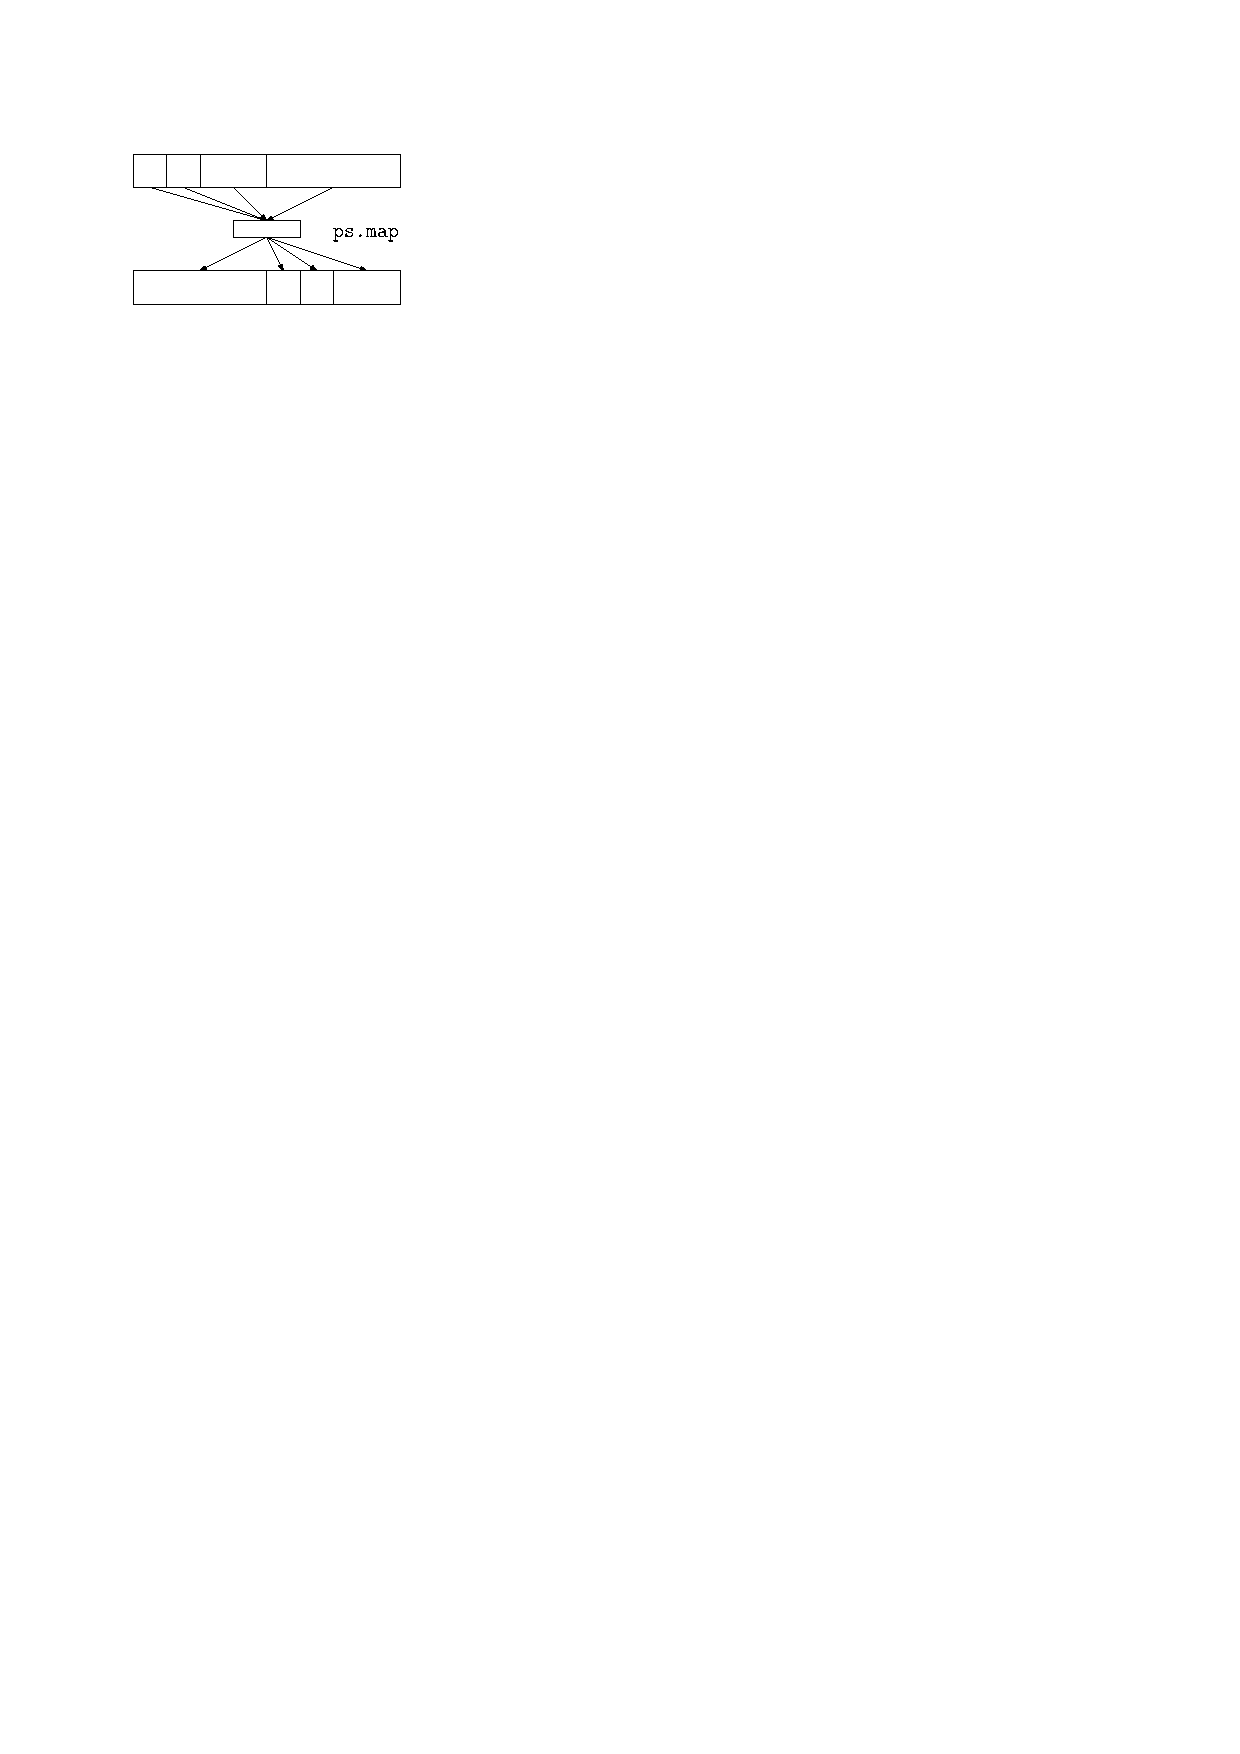
\includegraphics{barrier-free-pa}}
  \qquad
  \subfigure[FlowArray]{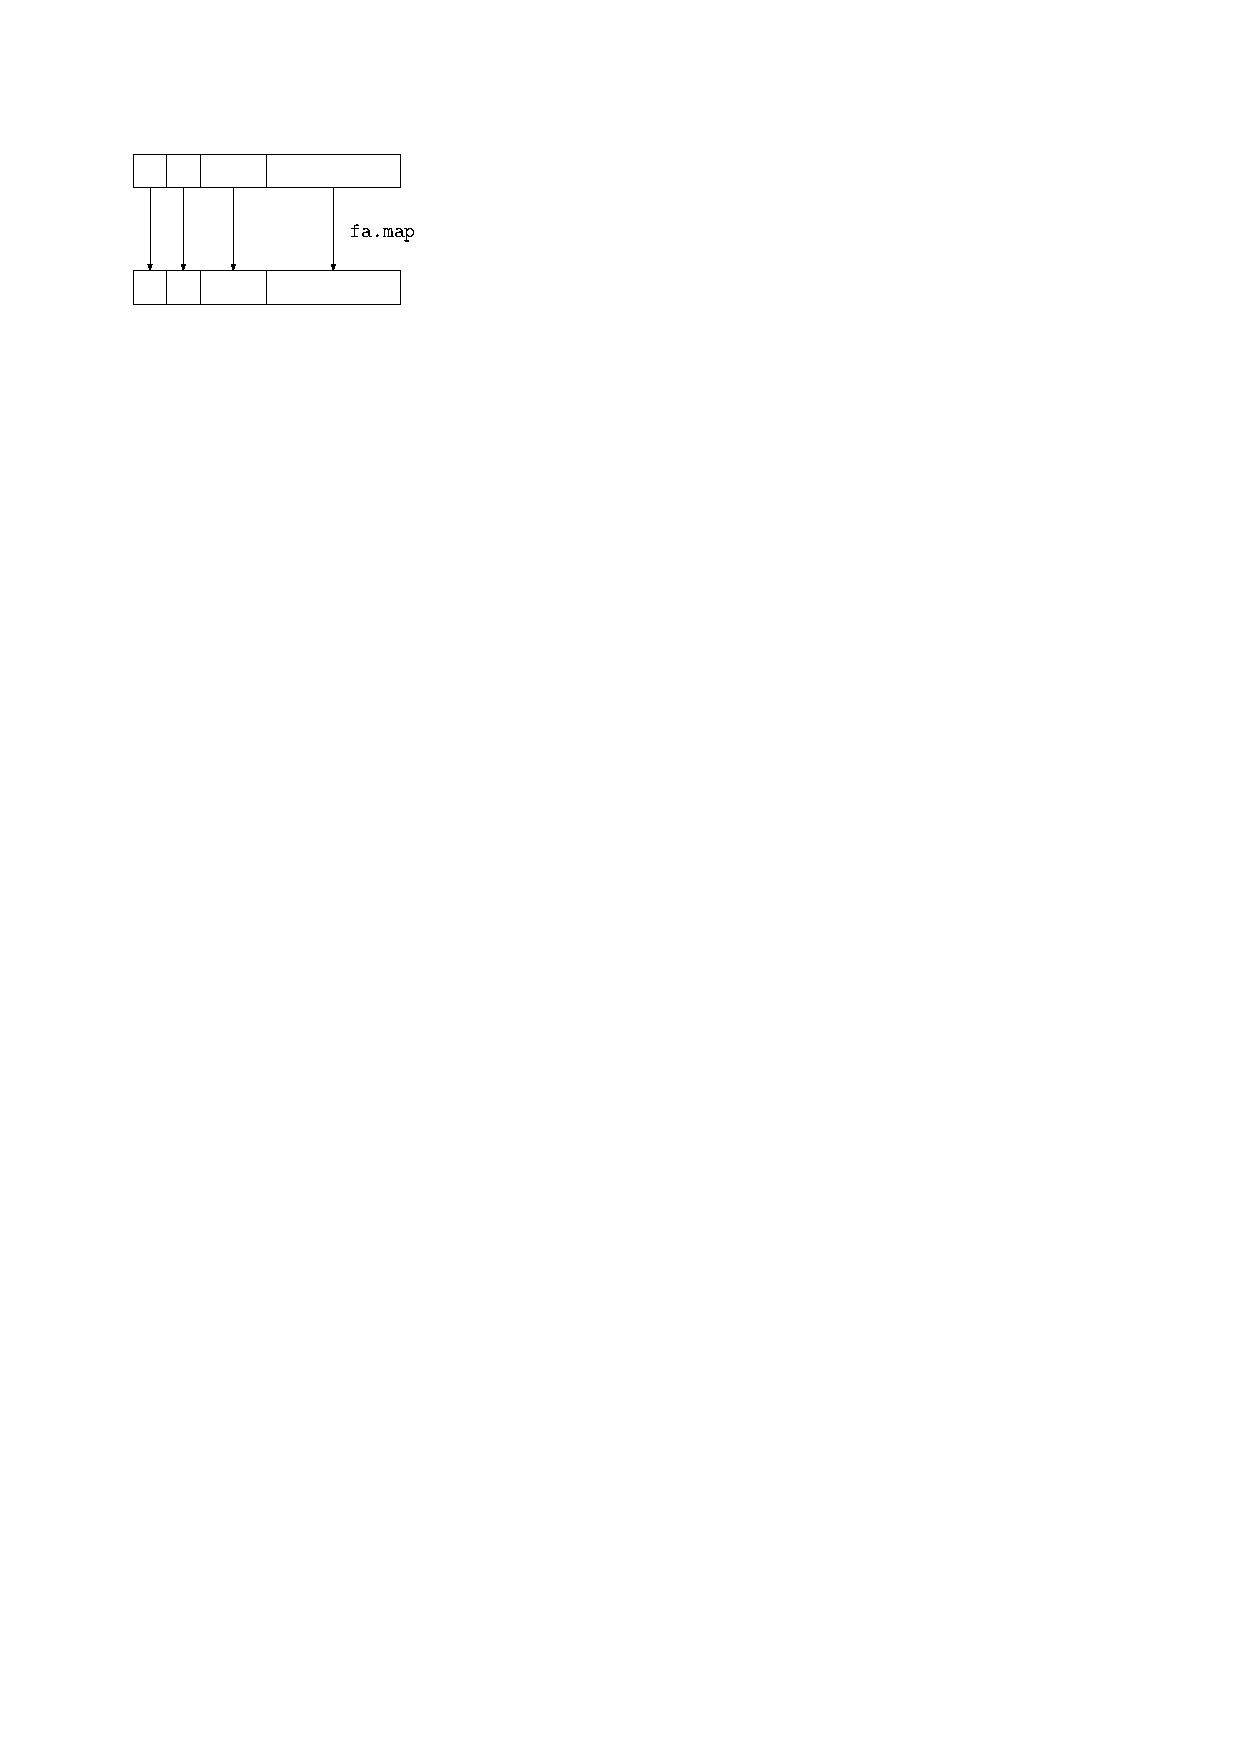
\includegraphics{barrier-free-fa}}
  \caption{Illustration of barrier-freedom of FlowArrays}
  \label{fig:barrier-free}
\end{figure}

\subsection{Dependency Tracking}


\section{Implementation}
\label{sec:implementation}

\subsection{FlowArray Jobs}

\subsection{Slice Views}

\subsection{Hierarchical FlowArrays}

\section{Evaluation}
\label{sec:evaluation}

\section{Conclusion}

\bibliographystyle{abbrv}
\bibliography{bib}

\end{document}

%%% Local Variables: 
%%% mode: latex
%%% TeX-master: t
%%% End: 
